\documentclass{article}

\usepackage{amsmath, graphicx}
\graphicspath{ {./images/} }

\title{Ch. 10 CW Solutions}
\author{Principles of Microeconomics}
\date{\today}

\begin{document}

\maketitle

\begin{enumerate}

\item

	\begin{enumerate}
	
	\item There's a positive externality because Mr. Chau's beautiful yard will make the whole neighborhood look better. That means the social value of his flowers is higher than their private value. The social cost is equal to the private cost because there are no external costs. Without intervention, there will be too little of the activity.
	
	\item There's a negative externality because the bonfires increase the risk of your house catching fire. The social value of the bonfires is equal to the private value because there is no external benefit to them. The social cost is higher than the private cost because of the negative externality. Without intervention, there will be too much of the activity.
	
	\item There's a positive externality because Maija's bees pollinate the apple orchard. That means the social value of her bees is higher than their private value. The social cost is equal to the private cost because there are no external costs. Without intervention, there will be too little of the activity.
	
	\item There's a negative externality because consuming a lot of gasoline creates a lot of $CO_2$ emissions. The social value of the SUV is equal to the private value because there are no external benefits. The social cost is higher than the private cost because of the negative externality. Without intervention, there will be too much of the activity.
		
	\end{enumerate}
	
\item

	\begin{enumerate}
	
	\item
		\begin{align*}
		\frac{1}{2}P_{mkt} &= 10 - 2P_{mkt} \\
		\frac{5}{2}P_{mkt} & = 10 \\
		P_{mkt} &= 4 \\
		Q_{mkt} &= \frac{1}{2}(4) = 2
		\end{align*}
		
	\item
	
		\begin{align*}
		\frac{1}{2}(P_{optimum} - 3) &= 10 - 2P_{optimum} \\
		\frac{5}{2}P_{optimum} &= \frac{23}{2} \\
		P_{optimum} &= \frac{23}{5} \\
		Q_{optimum} &= 10 - 2\left(\frac{23}{5}\right) \\
		Q_{optimum} &= \frac{4}{5}
		\end{align*}
		\begin{center}
		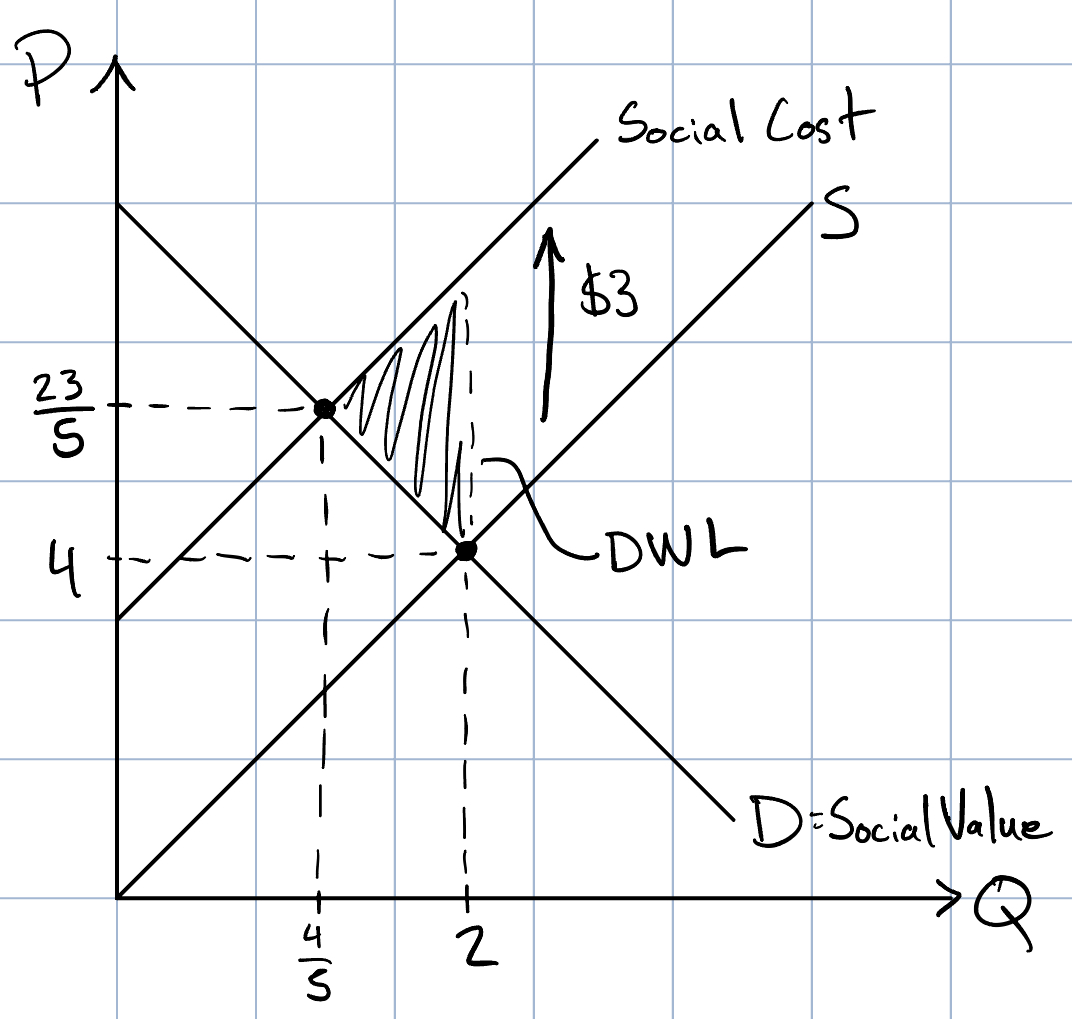
\includegraphics[width = 0.5\textwidth]{q2}
		\end{center}
		
	\item 
	
		\begin{align*}
		DWL &= \frac{3\left(2 - \frac{4}{5}\right)}{2} \\
			&= \frac{9}{5} 
		\end{align*}
	
	\end{enumerate}
	
\item

	\begin{enumerate}
	
	\item
	
		\begin{align*}
		4P_{mkt} &= 14 - 2P_{mkt} \\
		6P_{mkt} &= 14 \\
		P_{mkt} &= \frac{7}{3} \\
		Q_{mkt} &= 4\left(\frac{7}{2}\right) \\
		&= \frac{28}{3}
		\end{align*}
		
	\item
	
		\begin{align*}
		4P_{optimum} &= 14 - 2(P_{optimum} - 2) \\
		6P_{optimum} &= 18 \\
		P_{optimum} &= 3 \\
		Q_{optimum} &= 4(3) \\
		&= 12
		\end{align*}
		
	\item The government could place a \$2 per unit subsidy on solar cells.
	
	\end{enumerate}
	
\item

	\begin{enumerate}
	
	\item The efficient outcome is Harmon ditching the dog because Andy values quiet more than Harmon values the dog.
	
	\item Andy would pay Harmon some amount between \$10,000 and \$20,000 to ditch the dog. Harmon would accept because he doesn't value the dog enough to keep it if he's receiving \$10,000+ to get rid of it. 
	
	\item Harmon would have to ditch the dog because he's not willing to pay the \$20,000 it would take to convince Andy to let him keep it.
	
	\item In both scenarios, Harmon ditches the dog, so it doesn't affect the dog's outcome. When Harmon has the right to keep the dog he gets paid. When he doesn't, no one gets paid.
	
	\end{enumerate}
	
\item

	\begin{enumerate}
	
	\item $130 \cdot \$5 + 20 \cdot \$2 = \$690$
	
	\item College Cleaners: \$5 \\
		Big Green Cleaners: \$2
		
	\item Big Green Cleaners will sell all of its vouchers to College Cleaners for some amount between \$2 and \$5. That's because College Cleaners is willing to pay Big Green Cleaners more than the \$2 that Big Green Cleaners values the vouchers.
	
	\item College Cleaners would have 200 permits, so they would only have to reduce their pollution by 30 units. That would generate a cost of $30 \cdot \$5 = \$150$. Big Green Cleaners has no permits, so they would have to reduce their pollution by 120 units. That would generate a cost of $120 \cdot \$2 = \$240$. In total, the cost of reducing pollution would be \$390 which is significantly less than the regulation in (a).
	
	\end{enumerate}

\end{enumerate}

\end{document}